\section{Dynamical Susceptibility and Excitations - Formalism for {\prg mcdisp}}
\label{formalism}

This section is describes the formalism used in the calculation of the magnetic excitations. Because the
procedure is not standard, we list the most important formulas.

We assume a quantum mechanical system that can be described by the Hamiltonian
 \begin{equation}\label{fullhamiltonian}
 \hat \mathcal H=\sum_{n=1}^N \hat \mathcal H(n) -\frac{1}{2} \sum_{n,n',\alpha,\beta}
 {\mathcal J}_{\alpha\beta}(\mbf R_{n'} - \mbf R_n) \hat \mathcal I_{\alpha}^n \hat \mathcal I_{\beta}^{n'}.
 \end{equation}
The first term $\hat \mathcal H(n)$ denotes the Hamiltonian of
 a subsystem $n$
(e.g.~an ion, or cluster of ions). The second term describes a bilinear interaction 
between different subsystems
through the operators $\hat \mathcal I_{\alpha}^n$, with $\alpha = 1,2,...,m$. The operators $\hat \mathcal H(n)$ and $\hat \mathcal I_{\alpha}^n$  act in the subspace $n$ of the Hilbert space, i.e. $[\hat \mathcal I_{\alpha}^n,\hat \mathcal I_{\alpha}^{n'}]=0$,
$[\hat \mathcal H(n),\hat \mathcal I_{\alpha}^{n'}]=0$ and $[\hat \mathcal H(n),\hat \mathcal H(n')]=0$
for $n \neq n'$\footnote{Note that these conditions are essential and put a  limit to the
applicability of the theory, for example in the case of charge transfer excitations from
one subsystem to the next\hili{~\cite{dagotto03-1}}.}.
For example, in the case of a Heisenberg
 exchange between magnetic ions we would identify the set of operators with
 $\alpha=1,2,3$ with the three components of the  spin: $\hat \mathcal I_1 \leftrightarrow \hat S_x, \hat \mathcal I_2 %%@
\leftrightarrow \hat S_y, \hat \mathcal I_3 \leftrightarrow \hat S_z$.
The beauty of the analysis which follows is that it can be applied to
almost any Hamiltonian of the form (\ref{fullhamiltonian}). The analysis
of complex magnetic systems can thus be attempted by starting from a simple
form such as the Heisenberg model and by introducing, step-by-step, more
complexity into the model. For example, anisotropy and interactions with extended range can be introduced by modifying ${\mathcal J}_{\alpha\beta}(\mbf R_n - \mbf R_{n'})$, higher order operators can be 
introduced  by extending the index range for $\alpha$, and a complex single-ion term $\hat \mathcal H(n)$ may be added. 
Another example for a Hamiltonian (\ref{fullhamiltonian})  is the problem of lattice dynamics, which can
 be treated in the framework of this
formalism by identifying the operators $\hat \mathcal I^n_{\alpha}$
 with the atomic displacements $u^{n}$. Here the index $\alpha$ is not necessary and
$n$ refers to both, the atomic position index and the spatial coordinate of the displacement,
  $n=(1,x),(1,y),(1,z),(2,x),(2,y),(2,z), ...$. Note that this can be done, because the three spatial components of the 
displacement operators commute with each other (in contrast to the components of the spin) and each displacement
component acts in its own subspace of the Hilbert space. The kinetic energy
will be part of the single ion term $ \hat \mathcal H(n)$. Allowing more complexity to the system,
both the spin and lattice degrees of freedom can be introduced and spin-phonon interactions can be
handled by the theory.

The main limitation of the approach is that it neglects fluctuations associated with phase 
transitions and quantum disorder. We are primarily concerned, therefore, with excitations 
associated with a  well-ordered ground state.

 The translational symmetry of the system is 
represented by a Bravais lattice (which, in general,
will be a superlattice of a crystal lattice). 
The position of subsystem $n$ can be specified by a lattice 
vector $\Bell$ and a basis vector $\mbf b_s$. The latter is 
the position of $n$ relative to $\Bell$. 
The index $s$ ($s=1,2,...,N_b$) labels the subsystems 
within the unit cell.

The calculation of the excited states of the
 system starts from a mean-field model for the ground-state order. 
We define a mean field acting on each subsystem by
\begin{equation}\label{meanfieldformula}
H_{\alpha}^s=\sum_{\Bell's'\beta}
 {\mathcal J}_{\alpha\beta}(\Bell'+\mbf b_{s'}-\Bell-\mbf b_s) \langle \hat \mathcal
I^{s'}_{\beta}\rangle,
\end{equation}
where $\langle \hat \mathcal I^{s'}_{\beta}\rangle$ represents the thermal expectation value at a temperature $T$ in the mean 
field acting on subsystem $s'$. Note that the mean field 
is periodic in the lattice, so does not depend on $\Bell$. 
The mean-field Hamiltonian for subsystem $s$ is then given by
\begin{equation}\label{mfhamiltonian}
\hat \mathcal H^{\rm MF}(s) =\hat  \mathcal H(s)
 - \sum_{\alpha=1}^m H_{\alpha}^s \hat \mathcal I^s_{\alpha}
\end{equation}
The mean-field ground state is obtained from the self-consistent solution of (\ref{meanfieldformula}) and (\ref{mfhamiltonian}). This iterative procedure is illustrated in fig.~\ref{figmfproc}. The mean field Hamiltonian (\ref{mfhamiltonian})
 for the subsystem $s$
is used to calculate the thermal 
expectation values 
$\langle\hat \mathcal I^{s'}_{\beta}\rangle$ 
for the initial mean field acting 
on all subsystems $s'=1,2, ...,m$. 
Equation~(\ref{meanfieldformula}) is then used to calculate 
a new set of mean fields. These are again 
used in (\ref{mfhamiltonian}), and the procedure 
repeated until convergence is reached to within
 some specified precision. The free energy of 
the mean field ground state is evaluated and 
compared to that of other solutions obtained
 at the same temperature (computed from other
initial states and superlattices). The solution with 
the lowest free energy corresponds to the stable ground state.



We now turn to the excited states. From linear response theory it can 
be shown~\cite[page 143]{jensen91-1}
that the excited states are poles of the dynamical susceptibility, 
which is defined by

\begin{equation}
\chi_{BA}^{}(\omega)=\lim_{\varepsilon\to0^+}\Bigg[\sum_{aa'}^{E_a\ne E_{a'}}
\frac{\langle a|\hat{B}|a'\rangle\langle a'|\hat{A}|a\rangle}
{E_{a'}-E_a-\hbar(\omega+i\varepsilon)}(n_a^{}-n_{a'}^{})
+\frac{i\varepsilon}{\omega+i\varepsilon}\chi_{BA}'(el)\Bigg]\label{generalsuszeptibility}
\end{equation}
where
\begin{equation}
\chi_{BA}'(el)=\frac{1}{kT}
\sum_{aa'}^{E_a= E_{a'}}\langle a|\hat{B}-\langle \hat{B}\rangle|a'\rangle \langle
a'|\hat{A}-\langle \hat{A}\rangle|a\rangle\,n_a^{}\label{e5}
\end{equation}
and
\begin{equation}
n_a^{}=\frac{\exp(-E_a^{}/kT)}{\sum_{a'}\exp(-E_{a'}/kT)};\qquad
\langle \hat{A}\rangle=\sum_a\langle a|\hat{A}|a\rangle\,n_a^{} \label{e6}
\end{equation}

Here the energy levels and eigenstates
 of the Hamiltonian (\ref{fullhamiltonian}) are denoted by $E_{\hili{a}}$ and
$|\hili{a} \rangle$, respectively.
$n_{\hili{a}}$ is the corresponding 
Boltzmann occupation probability. 
$\hat A$ and $\hat B$ are
quantum mechanical operators describing the perturbation 
to the Hamiltonian and the response of the system
according to the general concept of linear response theory~\cite{jensen91-1}.
The expression (\ref{generalsuszeptibility}) is based on a system with well defined
energy levels implying that the poles of
$\chi_{BA}^{}(z=\omega+i\varepsilon)$ are all lying on the real axis,
or that the absorptive part of the response function
\begin{equation}
\chi_{BA}''(\omega)\equiv\lim_{\varepsilon\to0^+}\frac{1}{2i}
\left[\chi_{BA}^{}(z)-\chi_{AB}^{}(-z^\ast)\right]\label{e7}
\end{equation}
becomes a sum of $\delta$-functions, which are only non-zero when
$\hbar\omega$ is equal to the excitation energies $E_{a'}-E_a$. If
the susceptibility contains an elastic contribution, then the
function $\chi_{BA}''(\omega)/\omega=\pi\chi_{BA}'(el)\delta(\omega)$
in the zero frequency limit. In any realistic, interacting system the
energy levels are no longer discrete states and fluctuations will
cause spontaneous transitions between the different levels. Nonzero
probabilities for such transitions may be accounted for in a
phenomenological way by replacing $E_{a'}-E_a$ in equation (\ref{generalsuszeptibility})
by $E_{a'}-E_a-i\Upsilon_{a'a}$, where $\Upsilon_{a'a}\ge0$. In this
approximation the response becomes a sum of Lorentzians
\begin{equation}
\chi_{BA}''(\omega)\simeq \sum_{aa'}
\frac{\langle a|\hat{B}|a'\rangle\langle a'|\hat{A}|a\rangle\,\Upsilon_{a'a}^{}}
{(E_{a'}-E_a-\hbar\omega)^2+\Upsilon_{a'a}^2}(n_a^{}-n_{a'}^{})
+\frac{\hbar\omega\,\Upsilon_0^{}}{(\hbar\omega)^2+\Upsilon_0^2}\chi_{BA}'(el)\label{e8}
\end{equation}
The same result is obtained if $\varepsilon$ is kept as a nonzero
positive quantity in (\ref{generalsuszeptibility}) instead of taking the limit
$\varepsilon\to0^+$, i.e.\ if assuming
$\varepsilon=\Upsilon_{a'a}/\hbar$ in the different terms in the sum
and $\varepsilon=\Upsilon_0/\hbar$ in the elastic term.

Because of the periodicity of our system we define generalized 
susceptibilities $\chi_{\alpha\beta}^{ss'}({\mbf Q},\omega)\equiv\chi_{BA}$ by choosing the Fourier transform operators
\begin{eqnarray}
\hat A&=&\frac{1}{\sqrt{N}}\exp({\rm i}{\mbf Q} \cdot \mbf b_{s'})\sum_{\Bell'}\exp({\rm i}\mbf Q  \cdot \Bell')\hat \mathcal I^{(\Bell' s')}_{\beta} \\
\hat B&=&\frac{1}{\sqrt{N}}\exp({\rm i}{\mbf Q}  \cdot \mbf b_{s})\sum_{\Bell}\exp({\rm i}\mbf Q  \cdot \Bell)\hat \mathcal I^{(\Bell s)}_{\alpha},
\end{eqnarray}
where $N$ is the number of unit cells.  It will also be convenient to introduce the Fourier transform of the two-body interaction
\begin{equation}
{\mathcal J}_{\alpha\beta}^{ss'}({\mbf Q})=\sum_{\Bell'} {\mathcal J}_{\alpha\beta}(\Bell'+\mbf
b_{s'}-\mbf b_s) \exp\{{\rm i}\mbf Q  \cdot (\Bell'+\mbf b_{s'}-\mbf b_s)\}
\end{equation}
We have arbitrarily chosen 
${\Bell} = 0$ since ${\mathcal J}({\mbf Q})$ 
is the same for all $\Bell$ due to the translational symmetry.

\begin{figure}[th]
\setlength{\unitlength}{0.14in} % selecting unit length
\centering % used for centering Figure
\begin{picture}(32,30) % picture environment with the size (dimensions)
% 32 length units wide, and 15 units high.
% Declares a diamond shape
\newsavebox{\diamondshape}
\savebox{\diamondshape}(8,12)
{
   \put(0,0){\line(3,1){7}}
   \put(0,0){\line(3,-1){7}}
   \put(14,0){\line(-3,1){7}}
   \put(14,0){\line(-3,-1){7}}
}
% Declares a parallelogram
\newsavebox{\parallelogramshape}
\savebox{\parallelogramshape}
{
   \put(0,0){\line(2,0){10}}
   \put(1.5,2.5){\line(2,0){10}}
   \put(0,0){\line(3,5){1.5}}
   \put(10,0){\line(3,5){1.5}}
}
%\newsavebox{\parallelogram}
\put(10,28){\usebox{\parallelogramshape}}
\put(12,29){initial $\langle\hat \mathcal I^{s'}_{\beta}\rangle$}
\put(16,28){\vector(0,-1){2}}
\put(6,23){\framebox(20,3){calculate mean fields using eqn.(\ref{meanfieldformula})}}
\put(16,23){\vector(0,-1){2}}
\put(17,21.75) {$H^s_{\alpha}$}
\put(6,18){\framebox(20,3){diagonalise $\hat \mathcal H^{\rm MF}(s)$, eqn.(\ref{mfhamiltonian})}}
\put(16,18){\vector(0,-1){2}}
\put(17,16.75) {$\epsilon_j,|j\rangle,p_j$}
\put(6,10){\framebox(20,6){
                \begin{tabular}{c} compute \\ thermal expectation values \\
				     $\langle\hat \mathcal I^{s'}_{\beta}\rangle=\sum_j p_j \langle j|\hat \mathcal I^{s'}_{\beta}|j\rangle$
				  \end{tabular}}}
\put(16,10){\vector(0,-1){1.5}}
\put(5,0.2){\usebox{\diamondshape}}
\put(10.2,5.9){convergence reached?}
\put(16,3.9){\vector(0,-1){1.5}}
\put(23.2,6.5) {no}
\put(17,3) {yes}
\put(23,6.2){\line(1,0){6}}
\put(29,6.2){\line(0,1){18}}
\put(30,15) {$\langle\hat \mathcal I^{s'}_{\beta}\rangle$}
\put(29,24){\vector(-1,0){3}}
\put(6,-0.6){\framebox(20,3){\begin{tabular}{c}compute free energy and \\ compare to other solutions \end{tabular} }}
\end{picture}
\caption{Illustration of the iterative flow used for solving the mean-field
Hamiltonian eq.~(\ref{mfhamiltonian})} % title of the Figure
\label{figmfproc} % label to refer figure in text
\end{figure}


The calculation of the dynamical 
susceptibility\footnote{the
\hl{$-$} on top of $\chi$ indicates matrix notation 
for $\chi_{\alpha\beta}^{ss'}$}  $\m{\chi}({\mbf Q},\omega)$
from the Hamiltonian (\ref{hamiltonian}) is carried out 
within the
mean field -- random phase approximation 
(MF--RPA)~\cite{jensen91-1,tjablikov67-1}. 
This approximation neglects correlations 
in the differences 
$ \hat \mathcal I^n(t) - \langle  \hat \mathcal I^n (t) \rangle $  of 
different subsystems $n$.
 In this approach the dynamical  
susceptibility $\m{\chi}({\mbf Q},\omega)$ 
for a primitive lattice ($s=s'=0$)
can be calculated from the solution to

\begin{equation}\label{mfrpasimple}
 1=\left [ \m{\chi}^0(\omega)^{-1}-\m{\mathcal J}({\mbf Q}) \right]\m{\chi}({\mbf Q},\omega),
\end{equation}

where $\m{\chi}^0(\omega)$ is the usual single ion magnetic
susceptibility tensor.
This equation can be written for the more general case of several
 subsystems ($s=1,2,3,4,...,N_B$) as

\begin{equation}\label{mfrpass}
\delta_{ss'}=
\sum_{s''=1}^{N_B}\left[
\delta_{ss''}[\m{\chi}^{s}(\omega)]^{-1}
-\m{{\mathcal J}}^{ss''}({\mbf Q})
\right]
\m{\chi}^{s''s'}({\mbf Q},\omega),
\end{equation}


\noindent or, in index notation, to

\begin{equation}\label{meanfieldrpa}
\delta_{ss'}\delta_{\alpha\beta}=
\sum_{s''=1}^{N_B}\sum_{\delta=1}^m\left[
\delta_{ss''}[\chi^{s}(\omega)]^{-1}_{\alpha\delta}
-{\mathcal J}_{\alpha\delta}^{ss''}({\mbf Q})
\right]
\chi_{\delta\beta}^{s''s'}({\mbf Q},\omega),
\end{equation}
where $\chi^{s}_{\alpha\beta}(\omega)$ is the
 subsystem susceptibility (the same for all $\Bell$), given by
\begin{equation}
\label{singleionsusceptibility}
\chi^{s}_{\alpha\beta}(\omega)=
\sum_{jj'} \frac{\langle j|\hat \mathcal I_{\alpha}-\langle\hat \mathcal I_{\alpha}\rangle|j'\rangle\langle j'|\hat \mathcal
I_{\beta}-\langle\hat \mathcal I_{\beta}\rangle|j\rangle}{\epsilon_{j'}-\epsilon_j-\hbar \omega}
(p_j-p_{j'}).
\end{equation}
where for the sake of simplicity we omit the $s$ index 
on all quantities on the right-hand side. 
Here $\epsilon_j$ and $\epsilon_{j'}$ are 
energy levels of the subsystem $s$ as calculated 
self-consistently within the mean-field theory
using the Hamiltonian (\ref{mfhamiltonian}), 
$|j\rangle$ and $|j'\rangle$ denote the corresponding 
eigenstates and $p_j$ the corresponding population numbers:
\begin{equation}
p_{j} = \frac{\exp(-\epsilon_{j}/\hl{k}T)}{\sum_{j'}\exp(-\epsilon_{j'}/\hl{k}T)}.
\end{equation}

The writing of (\ref{singleionsusceptibility}) has been simplified in two ways. The obvious
one is that $\omega$ should read $\omega+i \varepsilon$ where
$\varepsilon\to0^+$. Secondly, the elastic contribution is included
in (\ref{singleionsusceptibility}) by assuming the use of the following convention:
$\epsilon_{j'}$ is being replaced by $\epsilon_{j'}+d$ in all terms
where $\epsilon_{j'}=\epsilon_j$. The shift in energy introduced is
$|d|\ll k^{}T$ and hence
$p_j-p_{j'}=p_j\,d/k^{}T$ to leading order. Notice that
the matrix elements of the thermal expectation values in (\ref{singleionsusceptibility}) are
only nonzero in the special cases of $j=j'$. Using the two
conventions equation (\ref{singleionsusceptibility}) becomes 
equivalent to (\ref{generalsuszeptibility}) in the limit of
$d\to0$ (after taking the limit $\varepsilon\to0^+$).
Since the expectation values are only needed
in (\ref{singleionsusceptibility}) when considering the elastic contribution, we may use this
fact to signal that the second convention has to be applied whenever
the expectation values are subtracted from the operators.

In order to evaluate
 equations
(\ref{mfrpasimple})-(\ref{singleionsusceptibility}) without producing a numerical divergence 
it is necessary to add to $\omega$ a small imaginary constant $\omega \rightarrow \omega+i\epsilon$
and insert this into equation (\ref{singleionsusceptibility}). 
If the option {\prg -r $\epsilon$} is used,
the program {\prg McDisp} calculates the above expression for every energy
and stores the result in {\prg ./results/mcdisp.dsigma}. 

 If the option {\prg -r} is not used, the
 program {\prg mcdisp\index{mcdisp}} uses only the extremely fast DMD (Dynamical Matrix Diagonalisation) %%@
algorithm\cite{rotter06-400} to calculate excitation energies and intensities and store the result in {\prg mcdisp.qom, %%@
mcdisp.qei, etc.}. The flowing chart of such a calculation is shown in fig.~\ref{figdmdproc}
and the formalism is outlined hereafter:


\subsection{DMD - formalism}\label{DMDform}

The central problem in applying the MF--RPA is the calculation of the
dynamical susceptibility 
$\chi_{\delta\beta}^{s''s'}({\mbf Q},\omega)$ 
from equation ~(\ref{meanfieldrpa}).
The standard procedure is to substitute equation~(\ref{singleionsusceptibility}) 
into~(\ref{meanfieldrpa}), which is 
then solved for each desired value of $\omega$ and ${\bf Q}$ by a matrix
inversion. In order to avoid a numerical divergence,
% it is necessary to add
%to $\hbar \omega$ a small imaginary constant $\hbar \omega \rightarrow \hbar
%\omega + i \hbar \varepsilon$ and insert this into equation (\ref{singleionsusceptibility}).
 \hl{it is necessary to add to $\hbar\omega$ a small imaginary
constant $\hbar\omega\to\hbar\omega +i\Upsilon$ and insert this into
equation (\ref{singleionsusceptibility}) leading to a susceptibility which is equivalent to 
equation (\ref{e8}). }
This method is inefficient and time demanding, however , because a $3N_b\times 3N_b$ matrix has to
be inverted for each $(Q,\omega)$ in the calculation.

In order to minimise the computational
effort an algorithm was developed \cite{rotter06-400}, which requires only the solution
of a single generalised eigenvalue problem at each scattering vector $\mbf Q$.
This dynamical matrix diagonalisation (DMD) resembles the standard approach
to lattice dynamics. % and is summarised in the next section.
This approach is very fast and will allow for more complex 
systems to be investigated\footnote{supplementary material - screen
shot movie comparing the speed of traditional Green's function method and DMD}.

In the following we describe the DMD
 for a single excitation \hili{ $\epsilon_- \rightarrow \epsilon_+$ }
of each 
subsystem $s$, i.e.
we assume that each subsystem is a two level system
\hili{with a single transition only}. 
Other transitions 
\hili{(terms in equation (\ref{singleionsusceptibility}))}
can be considered in the DMD formalism
 by assigning
to each of these transitions an additional value
 of the index $s$ and increasing the total number 
of subsystems ($N_b$) correspondingly. This
procedure is different from adding other terms 
(which are present in equation~(\ref{singleionsusceptibility}))
to the right hand side of equation (\ref{sisusc}). 
However, both procedures lead to the same results, 
this is shown in~\cite{rotter12-213201}.

\hili{For readability it is convenient to adopt the following
matrix notation: a $m \times m$ matrix is indicated by 
\hl{a bar} on top of the symbol, e.g. $\m{\chi}^s$
refers to the matrix $\chi_{\alpha\beta}^s$ with 
$\alpha,\beta=1,\dots,m$. A $N_b \times N_b$ matrix is 
denoted by \hl{a bar} below the symbol. 
Making use of these two conventions
the dynamical susceptibility 
$\chi_{\alpha\beta}^{ss'}({\mbf Q},\omega)$ can be
written as $\m{\M{\chi}}({\mbf Q},\omega)$.
}

Considering only a single 
excitation \hili{$\epsilon_- \rightarrow \epsilon_+$} in 
the subsystem susceptibility, equation~(\ref{singleionsusceptibility}) 
can be rewritten as

\hili{
\begin{equation}\label{sisusc}
\m{\chi}^{s}(\omega)=
\frac{\m{M}^s}{\Delta^s-\hbar \omega}
\end{equation}
}

\noindent with $\Delta^s\equiv\epsilon^s_+-\epsilon^s_-$ and
 the transition \hili{element matrix}

\begin{equation}\label{mmatrix}
M^s_{\alpha\beta}=\langle-|\hat \mathcal I^s_{\alpha}-\langle\hat \mathcal I^s_{\alpha}\rangle|+\rangle\langle+|\hat \mathcal %%@
I^s_{\beta}-\langle\hat \mathcal I^s_{\beta}\rangle|-\rangle
(p_--p_+)
\end{equation}

{\tiny Note for experts on programming single ion modules: that any external single ion module has to provide the 
matrix $M^s_{\alpha\beta}$ for every transition
$|-\rangle \rightarrow |+\rangle$which is to be taken into consideration in the calculation. If the energy of this transition
is zero, i.e. $\Delta^s=0$ (diffuse scattering), the expression (\ref{mmatrix}) would be zero because $(p_--p_+)$ 
vanishes.
In this case the single ion module should calculate $(p_+/kT)$ instead of $(p_--p_+)$.
}

 The $m \times m$  matrices \hili{ $\m{M}^s$} may be diagonalised giving eigenvalues which are all zero
except for one
\hili{real} eigenvalue $\gamma^s$ 
\hili{(which has the same sign as $\Delta^s$)}:

\hili{
\begin{equation}
 \gamma^s=\Trace{\m{M}^s}
\end{equation}
}

Now, the MF--RPA  problem (\ref{mfrpass}) may be simplified by using
the unitary transformation
\hili{ ${\m{\mathcal U}^s}$ (${\m{\mathcal U}^{s\dag}\m{\mathcal U}^s}=\m{1}$),
 which diagonalises $\m{M}^s$.}
 Note that the first column of this matrix \hili{
 $\m{\mathcal U}^s$ } (the eigenvector with the 
eigenvalue $\gamma^s$) is simply

\begin{equation}\label{ufirstrow}
{\mathcal U^s_{\alpha1}}=\sqrt{(p_--p_+)/\gamma^s}\langle-|\hat \mathcal I^s_{\alpha}-\langle\hat \mathcal I^s_{\alpha}\rangle_{\mbf %%@
H,T}|+\rangle
\end{equation}

 This property is useful as most of the equations below require 
only knowledge of this first column. Following the 
procedure outlined in~\cite{rotter06-400} one may transform
 the subsystem interaction ${\mathcal J}_{\alpha\beta}^{ss'}({\mbf Q})$
\hili{
\begin{equation}\label{jqtransform}
\m{\mathcal L}^{ss'}(\mbf Q) \equiv
\m{\mathcal U}^{s\dag}
\m{\mathcal J}^{ss'}({\mbf Q}) \m{\mathcal U}^{s'}
\end{equation}
}

Now the \hili{$N_b \times N_b$}
Hermitian dynamical matrix may be defined as

\hili{
\begin{equation}
A^{ss'}({\mbf Q})=\Lambda^{ss'}\Delta^s-\sqrt{\gamma^s} \mathcal L^{ss'}({\mbf Q}) \left (\sqrt{\gamma^{s'}} \right )^\ast
\end{equation}
}

\begin{figure}[th]
\setlength{\unitlength}{0.14in} % selecting unit length
\centering % used for centring Figure
\begin{picture}(40,40) % picture environment with the size (dimensions)
% 32 length units wide, and 15 units high.
\put(20,40)% puts everything with respect to the middle line top of the figure
{ %PUT 1
\savebox{\diamondshape} % declares a diamond question box
{
   \put(0,0){\line(3,-1){7.5}}
   \put(0,0){\line(-3,-1){7.5}}
   \put(0,-5){\line(3,1){7.5}}
   \put(0,-5){\line(-3,1){7.5}}
   \put(8,-1.9) {no}
   \put(7.4,-2.5){\line(1,0){8.6}}
   \put(-7,-5){\makebox(14,5){all $\mathbf{Q}$ calculated?}}
   %\put(0.5,-6.1) {yes}
   %\put(0,-5.0){\vector(0,-1){2}}
}
% Declares a parallelogram
\savebox{\parallelogramshape}
{
   \put(-5.5,-2.5){\line(2,0){10}}
   \put(-4,0){\line(2,0){10}}
   \put(-5.5,-2.5){\line(3,5){1.5}}
   \put(4.5,-2.5){\line(3,5){1.5}}
}
\usebox{\parallelogramshape}\makebox(0,-2.5){Diagonalise \hili{$\m{M}$}}
\put(1,-4.0){$\gamma^s,\hili{\m{\mathcal U}^s}$}
\put(0,-2.5){\vector(0,-1){2}}
\put(0,-4.5){ %PUT 2
             \put(-11,-2){\framebox(22,2){Transform \hili{$\m{\mathcal J}^{ss'}(\mathbf{Q})$ with
             $\m{\mathcal U}^s$}, eq.(\ref{jqtransform})}}
             \put(1,-3.15){\hili{$\M{\mathcal L}(\mbf Q)$}}
             \put(0,-2){\vector(0,-1){2}}
			 \put(16,-1){\vector(-1,0){5}}
\put(0,-4.0){ %PUT
             \put(-9,-2){\framebox(18,2){calculate \hili{$\M{A}({\mbf Q})$} and diagonalise}}
             \put(0,-2){\vector(0,-1){1.8}}
              \put(1,-3.15){$\hili{\omega^r},t^{r}$}
\put(-14.5,-3.0){ %PUTLEFT
              \put(-4.5,-7){\framebox(9,7){\begin{tabular}{c} Take the set of \\ observables $\hat \mathcal O_{\alpha}$, %%@
\\
			  calc. \hili{$\m{\nu}^s$}, eq.(\ref{numatrix}) \\ and diagonalise \end{tabular} }}
			}  % close PUTLEFT
\put(0,-4.0){ %PUT
              \put(-10,-2){\vector(1,0){4.5}} % vector from left
              \put(-9.5,-1.15){$\Gamma^s,\hili{\m{\mathcal{V}}^s}$}
              \put(-5.5,-4.5){\framebox(13,4.7){ \begin{tabular}{c}
			                calc. \hili{$\m{\M{X}}(\mbf Q,\hili{\omega^r})$ for} \\  modes
                                           \hili{$r=1,2,\dots,N_b$}\\ using eq.(\ref{Xcalc})\end{tabular}}}
              \put(0,-4.5){\line(0,-1){1.5}}
			  \put(0,-6){\line(1,0){7}}
			  \put(0,-6){\line(-1,0){7}}
              \put(-7,-6){\vector(0,-1){2}}
              \put(7,-6){\vector(0,-1){2}}
\put(-7,-8.0){ %PUTLEFT 1
			  \put(-6,-6){\framebox(12,6){\begin{tabular}{c} calculate correlation \\ function
                            \hili{$\m{\M{\Sigma}}(\mathbf{Q},\hili{\omega^r})$ }\\ of observables, %%@
eq.(\ref{fluctdissbeyond}) \end{tabular} }}
              \put(0,-6){\vector(0,-1){2}}
\put(0,-8.0){ %PUTLEFT
  			\put(-6.75,-2){\framebox(13.5,2){~calc. $S_{\mathrm{mag}}^{\mathrm{inel}}(\mathbf{Q},\hili{\omega^r})$,
			  eq.(\ref{sinelmag}) }}
             \put(0,-2){\line(0,-1){2}}
             } }% close PUTLEFT
%            1 2 3 4 			
\put(+7,-8.0){ %PUTRIGHT 1
               \put(-6,-4){\framebox(12,4){\begin{tabular}{c} calc. $\Delta\langle\mathcal{O}_\alpha^n \rangle$\\
                                           eq.(\ref{oscillation}) \end{tabular}}}
               \put(0,-4){\vector(0,-1){2}}
\put(+0,-6.0){ %PUTRIGHT
              \put(-6,-2){\framebox(12,2){visualize modes}}
              \put(0,-2){\line(0,-1){4}}
             } }
%            1 2 3 4 	close PUTRIGHT		
\put(0,-20.0){ %PUT
			  \put(0,0){\line(1,0){7}}
			  \put(0,0){\line(-1,0){7}}
              \put(0,0){\vector(0,-1){2}}
              \put(0,-2.0){\usebox{\diamondshape}}
			  % line to return to box 2
			  \put(16,-4.5){\line(0,1){31.5}}
 } } } } }% close all puts
%1 2 3 4 5 6 7 8 9
%\put(0,-4.0){ %PUT
%              \put(-11,-2){\framebox(22,2){ use $\hili{\omega^r},t^{r}$
	%		                to calculate $\chi_{\alpha\beta}^{ss'}(\mbf Q,\omega)$}}
     %         \put(0,-2){\vector(0,-1){2}}
\end{picture}
\caption{Illustration of the DMD procedure (see sections \ref{DMDform} and \ref{chiobservable} of text).} % title of the Figure
\label{figdmdproc} % label to refer figure in text
\end{figure}



The energies of the system may be calculated by solving the following
generalised eigenvalue problem:

\hili{
\begin{equation}\label{evproblem}
\M{A}({\mbf Q})\mbf{t}=\hbar\omega \M{\Lambda} \mbf{t}
\end{equation}
}

\noindent where the matrix \hili{$\M{\Lambda}$} is defined as

\hili{
\begin{equation}\label{lambdass}
\Lambda^{ss'}=\delta_{ss'}{\rm sgn}(\Delta^s)
\end{equation}
}

The solution of the generalised eigenvalue problem (\ref{evproblem}) yields
the eigenvectors \hili{$\M{\mathcal T}=\left( \mbf t^1, \mbf t^2, \dots,\mbf t^r,\dots\right)$ and eigenvalues $\hbar \omega^r$}.
These may be written as the eigenvalue matrix 
\hili{$\Omega^{rr'}=\delta_{rr'}\hbar \omega^r$}, and correspond %%@
to the excitation energies of the system at the wavevector
 ${\bf Q}$ for which \hili{$\M{A}({\mbf Q})$} was calculated.
The solution of the eigenvalue problem (\ref{evproblem}) corresponds to the %%@
diagonalisation of the dynamical matrix in the case of phonons and therefore this method for calculating magnetic %%@
excitations is called dynamical matrix diagonalisation (DMD).
 Note, that the matrix \hili{$\M{A}({\mbf Q})$} does not change
when the number of dimensions $m$ of the subsystem susceptibility is increased (for example to include quadrupolar degrees %%@
of freedom), unless there is an interaction coupling these degrees of freedom between different ions (this can be seen %%@
by the definition (\ref{jqtransform}) of the matrix 
\hili{$\M{\mathcal L}$} having in mind the first column of the %%@
transformation
matrices \hili{$\m{\mathcal U}^s$}, see equation (\ref{ufirstrow})).

The eigenvector matrix \hili{$\M{\mathcal T}$} provides a 
unitary transformation, which may be used to obtain the
 dynamical susceptibility. 
If the eigenvectors are normalised as
\hili{$\M{\mathcal T}^\dag \M{A}\M{\mathcal T}=\M{1}$}, then
equation (\ref{meanfieldrpa}) may be transformed using \hili{$\m{\mathcal U}^s$}
 and \hili{$\M{\mathcal T}$}(see~\cite{rotter12-213201}):

\begin{equation}\label{dmdfinal}
\chi^{ss'}_{\alpha\beta}(\mbf Q,\omega)=\left (\sqrt{\gamma^{s}} \right )^\ast \sum_r
\mathcal U^s_{\alpha1} \hili{\mathcal T^{sr}(\mbf Q) \frac{\hbar \omega^r(\mbf Q)}{\hbar \omega^r(\mbf Q) %%@
- \hbar \omega} \mathcal T^{rs'\dag}(\mbf Q)} \mathcal U^{s'\dag}_{1\beta}\sqrt{\gamma^{s'}}
\end{equation}

By its definition the generalised susceptibility gives information about the correlated
movement of the operators $\langle \hat \mathcal I_{\alpha}^s \rangle $
for a specific excitation and contains the relative phases and amplitudes of the
different operators.
The procedure for the calculation of excitation energies \hili{$\hbar\omega^r$} and physical
 observables (such as correlation functions and spectra) outlined above is very fast, because it
involves only a single diagonalisation (determination of the
 matrix \hili{$\M{\mathcal T}$}) for every scattering
vector of interest. The
dynamical susceptibility does not need to be calculated for each
 energy transfer by inverting equation
(\ref{mfrpass}) saving much
computation time. Therefore the module {\prg McDisp} of the {\prg McPhase} package
uses this method by default. We want to emphasize, that the procedure outlined in this section is general
and allows to treat any number and combination of multipolar interactions just by
letting the index $\alpha$ in $\hat \mathcal I_{\alpha}^n$ take values between 1  and the number
of multipolar operators considered ($\alpha=1,\dots,m$).

Figure~\ref{figdmdproc} illustrates the DMD algorithm. We have described the first three parts
shown in the figure, obtaining the eigenvectors \hili{$\mbf t^{r}$}
 and eigenvalues \hili{$\omega^r$}. The following
parts are described in the next section where the 
dynamical susceptibility \hili{$\m{\M{\chi}}(\mbf Q,\omega)$}
is used to calculate a general susceptibility
 \hili{$\m{\M{X}}(\mbf Q,\omega)$} corresponding
to an arbitrary observable, from which physical properties may be calculated.


\subsection{Calculation of the Correlation Function of Physical Observables}
\label{chiobservable}

 Physical observables are related to operators such as the magnetic moment components or the scattering operators. We now
introduce a series
of observables $\hat \mathcal O_{\alpha}$ ($\alpha=1,...,m'$)
for each subsystem $n=(\Bell s)$
and define a corresponding correlation function and
dynamical susceptibility. The correlation function we denote as
\hili{$\M{\m{\Sigma}}({\mbf Q},\omega)$}

\begin{eqnarray}\label{sigmass}
\hili{\Sigma^{ss'}_{\alpha\beta}}({\mbf Q},\omega)&=&\int_{-\infty}^{+\infty}dt e^{i\omega t}e^{-i\mbf Q \cdot(\mbf b_s-\mbf %%@
b_{s'})}
\frac{1}{N_g}\sum_{\Bell \Bell'}e^{-i\mbf Q \cdot(\Bell-\Bell')} \times \nonumber \\
&& \times(\langle \hat \mathcal O^{\Bell s \dag}_{\alpha}(t) \hat \mathcal O^{\Bell' s'}_{\beta}(0) \rangle_{T,H}
- \langle \hat \mathcal O^{\Bell s \dag}_{\alpha}\rangle_{T,H} \langle \hat \mathcal O^{\Bell' s'}_{\beta} %%@
\rangle_{T,H})
\end{eqnarray}

Note that the observables $\hat \mathcal O_{\alpha}^{\Bell s}$ may have some $\mbf Q$ dependence (for example if we
consider the Fourier transform of a magnetisation density of
 a magnetic ion in a crystal~\hili{\cite{balcar89-1}}). We
omit this $\mbf Q$ dependence to make notation easier but will come back to it when considering
the calculation of the neutron scattering cross section.

Using the fluctuation-dissipation theorem
$\Sigma$ can be related to a dynamical susceptibility $X$:

\begin{equation}\label{fluctdissbeyond}
\hili{\M{\m{\Sigma}}}({\mbf Q},\omega) =
\frac{2 \hbar}{1-e^{-\hbar\omega/kT}}\left ( \hili{\M{\m{X}}} \right )''({\mbf Q},\omega)
\end{equation}

\begin{equation}\label{chiabs}
\left (X_{\alpha\beta}^{ss'}\right )''({\mbf Q},\omega)\equiv
\frac{1}{2i}\left[
X_{\alpha\beta}^{ss'}({\mbf Q},\omega)-
\hl{\left ( X_{\alpha\beta}^{ss'}({\mbf Q},\omega) \right )^{\ast}}
\right]
\end{equation}

However, in contrast to the dynamical susceptibility
\hili{$\M{\m{\chi}}$}, based
on the operators $\hat \mathcal I_{\alpha}$,
 the susceptibility \hili{$\M{\m{X}}$} 
cannot be obtained from solving the MF--RPA equation (\ref{meanfieldrpa}).
The reason is that the derivation of (\ref{meanfieldrpa})
makes use of the dynamical evolution of the operators $\hat \mathcal I_{\alpha}$
and not of the observables $\hat \mathcal O_{\alpha}$.

Nonetheless, general properties of dynamical susceptibilities may be used
to get a relation between
\hili{$\m{\M{X}}({\mbf Q},\omega)$ and
$\m{\M{\chi}}({\mbf Q},\omega)$}.
In general a dynamical susceptibility $\chi_{BA}(\omega)$ describes the response of
 a physical observable $\langle\hat B(t)\rangle$ to a perturbation of the system described by
an operator $\hat A$.
In the case of the dynamical susceptibility corresponding to the observables $\mathcal O_{\alpha}$ we therefore have to %%@
set $X_{\alpha\beta}^{ss'}({\mbf Q},\omega)\equiv\chi_{DC}(\omega)$ with the definitions

\begin{eqnarray}
\hat C=\frac{1}{\sqrt{N_g}}e^{i\mbf Q  \cdot\mbf b_{s'}}\sum_{\Bell'}e^{i\mbf Q \cdot\Bell'}\hat \mathcal O^{\mbf %%@
l's'}_{\beta} \\
\hat D=\frac{1}{\sqrt{N_g}}e^{i\mbf Q  \cdot\mbf b_{s}}\sum_{\Bell}e^{i\mbf Q \cdot\Bell}\hat \mathcal O^{\mbf %%@
ls}_{\alpha}
\end{eqnarray}

From linear response theory it can be shown~\cite[page 143]{jensen91-1}, that the dynamical
susceptibilities have poles at the excitation energies of the system: In equation ~(\ref{generalsuszeptibility})
the denominator, the eigenstates and the difference in thermal population are the same for any susceptibility.
The energy eigenstates $|\alpha \rangle$ of the system will be a linear combination of
direct products involving
single ion states.
Therefore, the numerator in equation (\ref{generalsuszeptibility}) will
be a (usually not known) linear combination of products of the form
$\langle -|\hat \mathcal I_{\alpha}^s|+\rangle \langle +'|\hat \mathcal I_{\beta}^{s'}|-'\rangle$
and
$\langle -|\hat \mathcal O_{\alpha}^s|+\rangle \langle +'|\hat \mathcal O_{\beta}^{s'}|-'\rangle$ for
 $\chi_{\alpha\beta}^{ss'}({\mbf Q},\omega)$ and
   $X_{\alpha\beta}^{ss'}({\mbf Q},\omega)$, respectively.

These terms can be related by a similar procedure to that
outlined in equations (\ref{mmatrix}) ff. We define the matrices,

\hili{
\begin{eqnarray}\label{mumatrix}
\mu^s_{\alpha\beta}=\langle-|\hat \mathcal I^{s}_{\alpha}-\langle \hat \mathcal I^{s}_{\alpha}\rangle|+\rangle\langle+|\hat \mathcal I^s_{\beta}-\langle \hat \mathcal I^s_{\beta}\rangle|-\rangle \\
\nu^s_{\alpha\beta}=\langle-|\mathcal O^{s \dag}_{\alpha}-\langle \mathcal O^{s \dag}_{\alpha}\rangle|+\rangle\langle+|\mathcal O^s_{\beta}-\langle \mathcal O^s_{\beta}\rangle|-\rangle \label{numatrix}
\end{eqnarray}
}

\noindent similar to the \hili{$\m{M}^s$} of equation~(\ref{mmatrix}), however, omitting the 
thermal population factors and expectation values. These matrices
%the matrices  $\mu_{\alpha\beta}^s$ and $\nu_{\alpha\beta}^s$
can be diagonalised using the
unitary transformations \hili{$\m{\B \mathcal U}^s$ ($\m{\B \mathcal U}^{s\dag}\m{\B \mathcal U}^s=\m{1}$) 
and
$\m{\B \mathcal V}^s$ ($\m{\B \mathcal V}^{s\dag}\m{\B \mathcal V}^s=\m{1}$)}, respectively.


Again, all eigenvalues are zero except for 
$\phi^s$ and $\xi^s$, respectively.

\begin{equation} \label{phieig}
\phi^s \equiv \B \gamma^s/(p_--p_+)=\hili{\rm Trace \{\m{\mu^s} \} }
\end{equation}
\begin{equation} \label{xieig}
\xi^s \equiv \Gamma^s /(p_--p_+) =\hili{\rm Trace \{\m{\nu^s} \} }
\end{equation}

In~\cite{rotter12-213201} these transformations
are used to derive the following expression for the
dynamical susceptibility 



\begin{equation}\label{Xcalc}
X^{ss'}_{\alpha\beta}=(\sqrt{\Gamma^s})^\ast
 \sum_r
\mathcal V^s_{\alpha1} \hili{\mathcal T^{sr} 
\frac{\hbar \omega^r}{\hbar \omega^r %%@
- \hbar \omega} \mathcal T^{rs'\dag}} \mathcal V^{s'\dag}_{1\beta} \sqrt{\Gamma^{s'}}
\end{equation}

% REMOVED BECAUSE in GEN SUSC TH EXP INCLUDED DUE TO COMMENTSOf REFEREE 2
%with the definition
%\footnote{If $\langle+|\neq\langle-|$ then $\m{\B \mathcal V}^s=\m{\mathcal V}^s$.}

%\begin{equation}
% \mathcal V^s_{\alpha1} \equiv \B \mathcal V_{\alpha1}^s
%\sqrt{\frac{\gamma^s}{\B \gamma^s}}^{\ast}
%\sum_{\alpha''=1}^m  \B \mathcal U^{s\dag}_{1\alpha''}
%\mathcal U^s_{\alpha''1}
%\end{equation}


Equation (\ref{Xcalc}) shows how knowledge of the dynamical susceptibility calculated
on the basis of the interaction operators between subsystems ($\hat \mathcal I_{\alpha}^s$)
may be used to obtain the dynamical susceptibility for any set of observables $\hat \mathcal O_{\alpha}$  of
the system. 

The standard procedure to avoid divergences is to substitute $\hbar \omega$ with $\hbar \omega + i \hbar \varepsilon$ and
take the limit for $ \varepsilon \rightarrow 0^+$. Using Dirac's formula 

\begin{equation}\label{dirac}
\lim_{ \varepsilon \rightarrow 0^+} 
\frac{1}{\hbar \hili{\omega^r}-\hbar \omega -i\hbar \varepsilon}=
\mathcal P \frac{1}{\hbar\hili{\omega^r} - \hbar \omega} +
 i \pi \delta(\hbar \hili{\omega^r} -\hbar \omega)
\end{equation}


\noindent the absorptive part of the dynamical susceptibility (\ref{chiabs}) becomes

\hili{
\begin{equation}\label{Xabscalc}
\left (X^{ss'}_{\alpha\beta}\right )''=\pi(\sqrt{\Gamma^s})^\ast
 \sum_r \mathcal V^s_{\alpha 1} \mathcal T^{sr} \hbar \omega^r 
\delta(\hbar \omega^r
- \hbar \omega) \mathcal T^{rs'\dag}(\mbf Q) 
\mathcal V^{s'\dag}_{1\beta} \sqrt{\Gamma^{s'}}
\end{equation}
}

\noindent and the correlation function \hili{$\M{\m{\Sigma}}$} can be evaluated by applying the 
fluctuation dissipation theorem (\ref{fluctdissbeyond}):

\begin{equation}\label{corrfunct}
\hili{\Sigma^{ss'}_{\alpha\beta}({\mbf Q},\omega)= 
\frac{2 \pi \hbar(\sqrt{\Gamma^s})^\ast\sqrt{\Gamma^{s'}}}
{1-e^{-\hbar\omega/kT}}
\sum_r
\mathcal V^s_{\alpha1} \mathcal T^{sr} \hbar \omega^r 
\delta(\hbar \omega^r
- \hbar \omega) \mathcal T^{rs'\dag} \mathcal V^{s'\dag}_{1\beta}}
\end{equation}

\hili{To keep notation simple, the $\mbf Q$ dependence of the eigenvectors
$\M{\mathcal T}$ and the energies $\omega^r$ has been omitted.
If the observable  $\hat \mathcal O_{\alpha}$ depends explicitly on $\mbf Q$, then also 
$\m{\nu}^s$ and thus $\m{\B \mathcal V}^s$ will depend on $\mbf Q$.}
This very fundamental result will be applied to the neutron scattering cross section
in section~\ref{formalism}.

\hl{
The elastic contribution to equations (\ref{Xabscalc}) and
(\ref{corrfunct}) has to be evaluated taking into account
a small but finite value for the energy shift $d$ introduced
in the discussion of equation (\ref{singleionsusceptibility}). It turns
out, that $\gamma^s$ and $\Gamma^s$ and thus also
the dynamical matrix $\M{A}$ and its eigenvalues
are proportional to $d$. Making use of the normalisation 
for the eigenvectors
$\M{\mathcal T}^\dag \M{A}(\mbf Q)\M{\mathcal T}=\M{1}$
we find that the dynamical susceptibility (\ref{Xabscalc})
is proportional to $d$ and thus zero in the limit of
$d \rightarrow 0$. However, in the  correlation function
(\ref{corrfunct}) the denominator is proportional to
$d$ leading to a finite result for the quasielastic response.
}

\subsection{Evaluating results - Graphical Visualisation of Spin and Charge Oscillations of %%@
Excitations}\label{visualization}

In section~\ref{chiobservable} we showed how to calculate the dynamical susceptibility and
the correlation function of observables by the DMD method. The eigenvalues of the generalised
eigenvalue problem (\ref{evproblem}) correspond to the excitation energies of the system at some wavevector ${\bf Q}$.
The eigenvectors may be used in equation (\ref{Xcalc}) to calculate for each excitation
the dynamical susceptibility.
This may be used to visualise the time or spatial dependence
of the observables (e.g. spins, angular moments, 
 charge density or atom positions etc.)
associated with such an excitation.

In linear response theory the dynamical susceptibility is derived by applying a perturbation to the
Hamiltonian (\ref{hamiltonian}) of the system, which is of the form

\begin{equation}
\hat \mathcal H_{\rm perturb}=\sum_{n',\beta} H^{n'}_{\beta}\hat  \mathcal O^{n'}_{\beta}
\end{equation}

 We assume a spatial and time dependent field of frequency $\omega$ and wavevector $\mbf Q$

\begin{equation}
 H^{n'}_{\beta}=H^{s'}_{\beta}
\exp(i\mbf Q \cdot \mbf R_{n'}-i\omega t), \qquad \mbf R_{n'}\equiv\Bell'+\mbf b_{s'}
\end{equation}

%Here we defined $\mbf R\equiv\mbf G_{l'}+\mbf b_{s'}$.

By virtue of its definition, the dynamical susceptibility describes
the response 
(change $\Delta \langle \hat \mathcal O_{\alpha} \rangle$
 of expectation values $\langle \hat  \mathcal O_{\alpha}\rangle$)
of the system in Fourier space:

\begin{equation}
\Delta \langle \hat  \mathcal O^s_{\alpha}\rangle(\mbf Q,\omega)=\sum_{s'\beta}X^{ss'}_{\alpha\beta}(\mbf Q,\omega) %%@
H^{s'}_{\beta}
\end{equation}

The corresponding oscillation of the moments $\langle \hat  \mathcal O_{\alpha}\rangle$ in real space and time is given %%@
by

\begin{equation}
\Delta \langle \hat \mathcal O^{n}_{\alpha}\rangle=
\Delta \langle \hat \mathcal O^s_{\alpha}\rangle(\mbf Q,\omega)
\exp(i\mbf Q \cdot\mbf R_{n}-i\omega t)=
\exp(i\mbf Q \cdot\mbf R_{n}-i\omega t) \sum_{s'\beta}X^{ss'}_{\alpha\beta}(\mbf Q,\omega) H^{s'}_{\beta}
\end{equation}

We eliminate the sum in this equation by choosing the components of the applied field $H^{s'}_{\beta}=H %%@
\delta_{1s'}\delta_{1\beta}$. In physical terms this means that we apply an oscillating field only to
the first component of the first subsystem (atom) in each unit cell and calculate the linear response
of all components of all subsystems (atoms) to this applied field:

\begin{equation}\label{osc}
\Delta \langle \hat \mathcal O^n_{\alpha}\rangle=
\exp(i\mbf Q \cdot\mbf R_{n}-i\omega t) X^{s1}_{\alpha1}(\mbf Q,\omega) H
\end{equation}

Due to the divergence of the susceptibility at the excitation ($\omega=\hili{\omega^r}$) a small
applied field $H$ will induce a large oscillation amplitude of the moments, the amplitude
of the oscillation will depend on the relation of magnitude of the applied field $H$ and
the rate of damping of the magnetic excitation. Therefore we set the amplitude $a_1$ of the
oscillation equal to $a_1=H/(\hbar\omega-\hbar\hili{\omega^r})$. Substituting this into (\ref{osc}) and
considering the susceptibility obtained from equation (\ref{Xcalc}) etc. we obtain

\begin{equation}\label{oscill}
\Delta \langle \hat \mathcal O^n_{\alpha}\rangle=
a_1 \exp(i\mbf Q \cdot\mbf R_{n}-i\hili{\omega^r} t)
\left (\sqrt{\Gamma^s}\right )^\ast \mathcal V^s_{\alpha1} 
\hili{\mathcal T^{sr}}(\mbf Q)\hbar \hili{\omega^r} 
 \hili{\mathcal T^{r1\dag}}(\mbf Q) %%@
\mathcal V^{1\dag}_{11}\sqrt{\Gamma^{1}}
\end{equation}

This procedure fails if \hili{$\mathcal T^{r1\dag}(\mbf Q)$} or
 $\mathcal V^{1\dag}_{11}$ is zero
which occurs when the mode $r$ of the subsystem
 $s=1$ does not change its moment $\langle \hat \mathcal O^1_1\rangle$. %%@
Therefore
it is convenient to redefine the amplitude 
$a=a_1 \hili{\mathcal T^{r1\dag}}(\mbf Q)  \mathcal %%@
V^{1\dag}_{11}\sqrt{\hbar \hili{\omega^r}\Gamma^{1}}$, giving

\begin{equation}\label{oscillation}
\Delta \langle \hat \mathcal O^n_{\alpha}\rangle=
a \exp(i\mbf Q \cdot\mbf R_{n}-i\hili{\omega^r} t)
\left ( \sqrt{\hbar \hili{\omega^r}\Gamma^s}\right )^\ast 
\mathcal V^s_{\alpha1} \hili{\mathcal T^{sr}}(\mbf Q) \equiv
a \exp(i\mbf Q \cdot\mbf R_{n}-i\hili{\omega^r} t) \hili{e^{s}_{\alpha}}
\end{equation}

If the eigenvector components $\hili{e^{s}_{\alpha}}$
 of this oscillation are stored for each mode $\hili{\omega^r}(\mbf Q)$, the
 dynamic fluctuation of this observable may be visualised in space and time
(files for the different observables are {\prg mcdisp.qem, mcdisp.qel, mcdisp.qes, mcdisp.qee, ...}).
In this way it is possible to produce figures and animated movies of spin or charge
density oscillations. 

This is done  by the program {\prg display\_densities}
(see section\ref{displaydensities}), or step by step, by programs
{\prg spins} and {\prg javaview}.
A visualisation of the magnetic moment-oscillation can for example be created by
 commands {\prg spins -M T Ha Hb Hc h k l E} and {\prg java javaview 
model=results/spins.*.jvx Animation.LastKey=16}.
 Note in {\prg mcdisp.qem} the eigenvector components
for different $t$ in $s=(ijklt)$ 
(refering to different single ion transitions at the same ion $ijkl$)
 are summed up.

I order to visualize a charge density the eigenvector $e^s_{r\alpha}$
 indices $\alpha= 1,...,28$ refer to observables given by equation
(\ref{chargedensity_coefficients}) with $l$ even, which are used
to calculate the chargedensity according to equation (\ref{chargedensity_operator2})
in appendix~\ref{chargedensityoperator}.
The corresponding 
 oscillations 
$\Delta \langle \hat \mathcal O^n_{\alpha = (lm)}\rangle
=\Delta \langle\sum_i Z_l^{m}(\Omega_i)\rangle_n =
\Delta |p_{lm}| \theta_{l} \langle O_l^m(\mbf J_n)\rangle$
 can be directly inserted into
(\ref{chargedensity2}) in order to evaluate the charge density oscillations. 
This is done by program
{\prg spins} with option {\prg -c},
 the commands are {\prg spins -c -M T Ha Hb Hc h k l E} and {\prg java javaview 
model=results/spins.*.jvx Animation.LastKey=16}. 
Fig.~\ref{animationAF1} shows a snapshot of the result of such an 
animation (on screen both chargedensities and spins will move).

\begin{figure}[tb]%h=here, t=top, b=bottom, p=separate figure page
\begin{center}\leavevmode
\includegraphics[angle=0, width=0.6\textwidth]{figsrc/dispF1.eps}
\end{center}
\caption{\label{dispF1}NdCu$_2$ Magnetic Excitations [meV] along ($h$00) in the phase F1 in comparison to experimental %%@
data~\cite{rotter02-751}.}
\end{figure}

\begin{figure}[tb]%h=here, t=top, b=bottom, p=separate figure page
\begin{center}\leavevmode
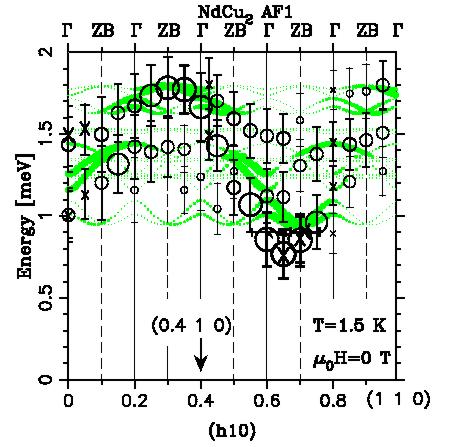
\includegraphics[angle=-0, width=0.6\textwidth]{figsrc/dispAF1.eps}
\end{center}
\caption{NdCu$_2$ Magnetic Excitations [meV] along ($h$00) in the phase AF1 in comparison to experimental %%@
data~\cite{rotter02-751}.}
\end{figure}

\begin{figure}[ht]%h=here, t=top, b=bottom, p=separate figure page
\begin{center}\leavevmode
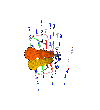
\includegraphics[angle=-0, width=0.6\textwidth]{figsrc/animationAF1.eps}
\end{center}
\caption{NdCu$_2$ - snapshot of animation of the mode 
at Q=(0.67 1 0) at energy 0.7~meV in phase AF1 at 
H=0 and T=1.5~K [plot created by program 
{\prg display\_densities}\index{display\_densities}]
}\label{animationAF1}
\end{figure}

\subsection{Application to Neutron scattering}
\label{neutronformalism}

We now apply the theory outlined above to the inelastic scattering of neutrons 
in a crystalline solid. The observables measured here are the atomic displacement (for phonons) and the
Fourier transform of the magnetisation (=magnetic moment density) operator of a magnetic ion ($\hat \mbf M(\mbf Q)$).
The magnetisation operator consists of a spin and an orbital contribution and thus
its Fourier transform may be written as a sum $\hat \mbf M(\mbf Q)=\hat \mbf M_S(\mbf Q)+\hat \mbf M_L(\mbf Q)$.
For consistency with ref.\cite{lovesey84-1} please note that we write the following formulas 
in terms of the magnetisation operator instead of the scattering operator
$\hat \mathcal Q_{\alpha} \equiv -\hat M_{\alpha}(\mbf Q)/(2\mu_B)$ (where $\alpha=x,y,z$ and $\mu_B$ is the
Bohr magneton).

The double differential neutron scattering cross section is usually being evaluated base on the master equation (see e.g. \cite{lovesey84-1})

\begin{equation}\label{masterequ}
\frac{d^2\sigma}{d\Omega dE'}=\frac{k'}{k}\left( \frac{m_n}{2\pi \hbar^2}  \right)^2
\sum_{if,s_n} P_{s_n} P_i \left | \langle s_n|\langle i|H_{int}(\mbf Q)|f\rangle|s_n'\rangle \right |^2 \delta(\hbar \omega+E_i-E_f)
\end{equation}

Here $m_n$ is the neutron mass, $\mbf k$ and $\mbf k'$ the incoming and scattered neutron wave vector, $|s_n\rangle$ and 
 $|s_n'\rangle$ the spin state of the incoming and scattered neutron, $P_{s_n}$ the polarisation of the incoming neutron
beam (i.e. the probability for the neutron spin state $|s_n>$ in the incoming neutron beam). $|i\rangle$ and $|f\rangle$ denote
the initial and final states of the target, $E_i$ and $E_f$ the corresponding energies, $P_i$ the population number
of the target state $|i\rangle$. Finally $H_{int}(\mbf Q)$ is the interaction operator which consists of neutron spin dependent
and spin independent parts

\begin{equation}
H_{int}(\mbf Q)=\hat \beta (\mbf Q) + \hat {\mbf s}_n \cdot \hat {\bm \alpha} (\mbf Q)
\end{equation}

Here $\hat \beta$ contains the nuclear spin independent scattering and $\hat {\bm \alpha}$ the nuclear spin dependent
and the electronic magnetic scattering operators.
The accurate evaluation of (\ref{masterequ}) involves the computation of terms $\hat \beta^{\dagger} \dots \hat \beta$ (nuclear scattering, phonons),
$\hat \alpha^{\dagger} \dots \hat \alpha$ (electronic magnetic scattering and nuclear magnetic scattering) 
and mixed terms $\alpha^{\dagger} \dots \beta$ (interference terms, not included in mcdisp currently, maybe nonzero only for
polarized beams).  We do not take into account any preferred occupancy of nuclear spin states in the sample, either.
Then the neutron intensity may be separated into nuclear (phonon) and magnetic intensity.
The corresponding expression for the double differential scattering cross section 
for unpolarised neutrons has been given frequently in literature (see e.g. \cite{lovesey84-1}):

%\begin{eqnarray}
%\frac{d^2\sigma}{d\Omega dE'}&=&N\frac{k'}{k}\left( \frac{\hbar \gamma e^2}{m_e c^2}  \right)^2
%%\sum_{\mbf Q} \delta_{\vec\kappa,\mbf Q}
%\sum_{\alpha\beta=1,2,3}(\delta_{\alpha\beta}- \frac{Q_{\alpha} Q_{\beta}}{|\mbf Q|^2}) 
%S^{\alpha \beta}_{\rm mag}(\mbf Q,\omega)+
%N\frac{k'}{k}S_{\rm nuc}(\mbf Q,\omega) \nonumber \\
%S_{\rm mag}&=&S_{\rm mag}^{\rm el}+S_{\rm mag}^{\rm inel} \label{smag} 
%\end{eqnarray}

%[BETTER USE THE FOLLOWING]
%\begin{eqnarray}\label{dsdoderepeated}
%\frac{d^2\sigma}{d\Omega dE'}&=&N\frac{k'}{k}\left( \frac{ \gamma r_0}{2 \mu_B}  \right)^2
%\sum_{\mbf Q} \delta_{\vec\kappa,\mbf Q}
%\sum_{\alpha\beta=1,2,3}(\delta_{\alpha\beta}- \frac{Q_{\alpha} Q_{\beta}}{|\mbf Q|^2}) 
%S^{\alpha \beta}_{\rm mag}(\mbf Q,\omega)+
%N\frac{k'}{k}S_{\rm nuc}(\mbf Q,\omega) \nonumber \\
%S_{\rm mag}&=&S_{\rm mag}^{\rm el}+S_{\rm mag}^{\rm inel} \label{smag} 
%\end{eqnarray}

\begin{eqnarray}\label{dsdoderepeated}
\frac{d^2\sigma}{d\Omega dE'}&=&
N\frac{k'}{k}S_{\rm nuc}(\mbf Q,\omega) +
N\frac{k'}{k} 
% \sum_{\alpha\beta=1,2,3} 
Tr\{S_{\rm mag\perp}(\mbf Q,\omega)\} \nonumber \\
S_{\rm nuc}&=&S_{\rm nuc}^{\rm el}+S_{\rm nuc}^{\rm inel} \label{snuc} \\ 
S_{\rm mag}&=&S_{\rm mag}^{\rm el}+S_{\rm mag}^{\rm inel} \label{smag} 
\end{eqnarray}


In (\ref{dsdoderepeated}) $N$ denotes the number of magnetic atoms in the sample, $\mbf k$ and $\mbf k'$ the wave vector %%@
of the incoming and scattered neutron, respectively.
$\hbar \omega=E-E'$  and
$\mbf Q =\mbf k-\mbf k'$  denote the energy and momentum transfer.
The van Hove scattering functions $S_{\rm mag}$ and $S_{\rm nuc}$ may be split into an elastic and an inelastic part. We %%@
will discuss here only the inelastic scattering. 

\subsubsection{Coherent Nuclear Inelastic Scattering - 1 Phonon processes}

The coherent inelastic nuclear scattering (by phonons) is given by

\begin{eqnarray}\label{Snucinel}
S_{\rm nuc}^{\rm inel}(\mbf Q,\omega)&=&
\frac{1}{2\pi\hbar}\int_{-\infty}^{+\infty}dt e^{i\omega t}
\frac{1}{N}\sum_{nn'} b_n b_{n'} e^{-W_n(Q)- W_{n'}(Q)}\\
&\times&  e^{-i\mbf Q \cdot (\mbf R_n-\mbf R_{n'})}  
 (\langle  \mbf Q \cdot \hat {\mbf u}^{n}(t)  {\mbf Q} \cdot \hat{\mbf u}^{n'}(0) \rangle_{T,H}
\nonumber
\end{eqnarray}

 - here $b$ denotes the nuclear coherent scattering length and $\hat {\mbf u}$ the 
displacement. 
If we split the index $n$ into basis and 
lattice part $n=(\Bell,s)$ and 
compare equation~(\ref{sigmass}), we see that %%@
the nucler scattering function depends on the correlation function between the inner product of
scattering vector and displacement operator
$\mbf Q \cdot \hat \mbf u$, which is the observable in the case of coherent nuclear inelastic neutron scattering 
($\mathcal O \leftrightarrow b_s   e^{-W_s(Q)} \mbf Q \cdot\hat \mbf u^s$).

%may be treated by associating
%the observable $\mathcal O$ with $\mathcal O \leftrightarrow b e^{i\mbf Q \mbf u}$,
%, which is given by

\begin{eqnarray}
S_{\rm nuc}^{\rm inel}(\mbf Q,\omega)&=&\sum_{ss'} 
\frac{\hili{\Sigma^{ss'}}({\mbf Q},\omega)}{2\pi \hbar N_b} 
\end{eqnarray}

 $W_s(Q)$ is  the Debye-Waller
factor of the atom number $s$ in the  unit cell.
$N_b$ denotes the number of magnetic
atoms in the magnetic unit cell.
Therefore, if the generalised eigenvalue problem (\ref{evproblem}) for the dynamical matrix
has been solved, the nuclear neutron scattering function can
be  evaluated with the help of equations (\ref{fluctdissbeyond}) and (\ref{Xcalc}):

\begin{eqnarray}\label{sinelnucfinal}
S_{\rm nuc}^{\rm inel}(\mbf Q,\omega)&=&
\sum_{r,ss'}  
\frac{(\sqrt{\Gamma_{\rm nuc}^s(\mbf Q)})^\ast\sqrt{\Gamma_{\rm nuc}^{s'}(\mbf Q)}}
{N_b(1-e^{-\hbar\hili{\omega^r}(\mbf Q)/kT})} \times \\ \nonumber
&& \times \mathcal V^s_{{\rm nuc},\alpha1}(\mbf Q)
\hili{ \mathcal T^{sr}}(\mbf Q)\hbar \hili{\omega^r}(\mbf Q)
 \delta(\hbar \hili{\omega^r}(\mbf Q) - 
\hbar \omega) \hili{\mathcal T^{rs'\dag}}(\mbf Q) 
\mathcal V^{s'\dag}_{{\rm nuc},1\beta}(\mbf Q)
\end{eqnarray}

Once the eigenvectors \hili{$\M{\mathcal T}$} of the system have been determined, this expression can be 
 evaluated. {\prg mcdisp} evaluates for every mode the expression (\ref{sinelnucfinal}) with exception
of the $\delta$-function and multiplies it by $k'/k$ in order to get the nuclear Intensity $I_{\rm nuc}$ in
barns/meV formula unit.

\subsubsection{Magnetic inelastic Scattering}

Similar, the magnetic inelastic scattering is given by


%\begin{eqnarray}
%S_{\rm mag}^{\rm inel,\alpha\beta}(\mbf Q,\omega)&=&\frac{1}{2\pi\hbar}\int_{-\infty}^{+\infty}dt e^{i\omega t}
%\frac{1}{N}\sum_{nn'} e^{-W_r(Q)- W_{r'}(Q)} e^{-i\mbf Q(\mbf R_n-\mbf R_{n'})} \nonumber \\
%&&\times (\langle \hat \mathcal Q^{n \dag}_{\alpha}(t) \hat \mathcal Q^{n'}_{\beta}(0) \rangle_{T,H}
%- \langle \hat \mathcal Q^{n \dag}_{\alpha}\rangle_{T,H} \langle \hat \mathcal Q^{n'}_{\beta} \rangle_{T,H})
%\end{eqnarray}

%[BETTER USE THE FOLLOWING]


\begin{eqnarray}\label{Sinelperp}
S_{\rm mag\perp}^{\rm inel,\alpha\beta}(\mbf Q,\omega)&=&\left( \frac{ \gamma r_0}{2 \mu_B}  \right)^2
%(\delta_{\alpha\beta}- \frac{Q_{\alpha} Q_{\beta}}{|\mbf Q|^2}) 
\frac{1}{2\pi\hbar}\int_{-\infty}^{+\infty}dt e^{i\omega t}
\frac{1}{N}\sum_{nn'} e^{-W_n(Q)- W_{n'}(Q)}\\
&\times&  e^{-i\mbf Q \cdot (\mbf R_n-\mbf R_{n'})}   (\langle \hat M_{\perp\alpha}^{n \dag}(t,\mbf Q)  \hat M_{\perp\beta}^{n'}(0,\mbf Q) \rangle_{T,H}
- \langle \hat M^{n \dag}_{\perp\alpha}(\mbf Q)\rangle_{T,H} \langle \hat M^{n'}_{\perp\beta}(\mbf Q) \rangle_{T,H})\nonumber
\end{eqnarray}

The total magnetic cross section is $4\pi (\gamma r_0)^2=4\pi\left(\frac{\hbar \gamma e^2}{mc^2}\right)^2
=3.65$~barn. 
In (\ref{Sinelperp}) the first term in the bracket corresponds to the total and the second term to the elastic
scattering.
If we split the index $n$ into basis and 
lattice part $n=(\Bell,s)$ and 
compare equation~(\ref{sigmass}), we see that %%@
the scattering function depends on the correlation function between the magnetisation operator
$\hat \mbf M_{\perp}(\mbf Q)=\hat \mbf M(\mbf Q)-\mbf Q (\hat \mbf M_{\perp}(\mbf Q) \cdot \mbf Q)/Q^2$, which is the observable in the case of magnetic neutron scattering 
($\mathcal O \leftrightarrow \frac{ \gamma r_0}{2 \mu_B}  e^{-W(Q)} \hat \mbf M_{\perp}(\mbf Q)$).

\begin{equation}\label{sinelmag}
S_{\rm mag\perp}^{\rm inel,\alpha\beta}(\mbf Q,\omega)=
\sum_{ss'} 
  \frac{\hili{\Sigma^{ss'}_{\alpha\beta}}({\mbf Q},\omega)}{2\pi \hbar N_b} 
\end{equation}

 $W_s(Q)$ is  the Debye-Waller
factor of the atom number $s$ in the magnetic unit cell\footnote{In case
of magnetic order. In general this will be the unit cell of 
the Bravais lattice in section~\ref{formalism}, which
is a superlattice of the crystal lattice.}. $N_b$ denotes the number of magnetic
atoms in the magnetic unit cell.
Therefore, if the generalised eigenvalue problem (\ref{evproblem}) for the dynamical matrix
has been solved, the magnetic neutron scattering function can
be  evaluated with the help of equations (\ref{fluctdissbeyond}) and (\ref{Xcalc}):

\begin{eqnarray}\label{sinelmagfinal}
S_{\rm mag\perp}^{\rm inel,\alpha\beta}(\mbf Q,\omega)&=&
\sum_{r,ss'}  
\frac{(\sqrt{\Gamma_{\rm mag}^s(\mbf Q)})^\ast\sqrt{\Gamma_{\rm mag}^{s'}(\mbf Q)} }
{N_b(1-e^{-\hbar\hili{\omega^r}(\mbf Q)/kT})} \times \\ \nonumber
&& \times \mathcal V^s_{{\rm mag},\alpha1}(\mbf Q)
\hili{ \mathcal T^{sr}}(\mbf Q)\hbar \hili{\omega^r}(\mbf Q)
 \delta(\hbar \hili{\omega^r}(\mbf Q) - 
\hbar \omega) \hili{\mathcal T^{rs'\dag}}(\mbf Q) 
\mathcal V^{s'\dag}_{{\rm mag},1\beta}(\mbf Q)
\end{eqnarray}

Once the eigenvectors \hili{$\M{\mathcal T}$} of the system have been determined, this expression can be 
 evaluated. 
{\prg mcdisp} evaluates for every mode the expression (\ref{sinelmagfinal}) with exception
of the $\delta$-function and multiplies it by $k'/k$ in order to get the nuclear Intensity $I_{\rm nuc}$ in
barns/meV formula unit. In addition, the components of the magnetic scattering function
$S_{\rm mag}^{\rm inel,\alpha\beta}(\mbf Q,\omega)$ can be output (to be used to interpret
polarised magnetic neutron scattering).$\alpha,\beta$ then refer to either the xyz coordinate system
($y||b$,$z||(a \times b)$ and $x$ perpendicular to $y$ and $z$)
or the uvw coordinate system 
($\mbf u||\mbf Q=\mbf k- \mbf k'$,$\mbf w$ perpendicular to the scattering plane (as determined by the cross product of
subsequent vectors in the input q-vector list of {\prg mcdisp})
 and $\mbf v$ perpendicular to $\mbf u$ and $\mbf w$, such that uvw for a righthanded system).

Form factor effects on the scattering intensity are
 due to the $\mbf Q$-dependence of the magnetisation operator, which means that
the transformation matrices \hili{$\m{\mathcal V}^s$}
 and the eigenvalues $\Gamma^s$ are also
$\mbf Q$-dependent.  These quantities have
 to be calculated by evaluating the transition
matrix elements\footnote{\hili{using the appropriate 
expression for the matrix elements of of the scattering
operator as given in~\cite[equ. (11.86) or (11.87b)]{lovesey84-1}.}} 
of \hili{$\hat \mbf M_{\perp}(\mbf Q)$ for every 
scattering vector $\mbf Q$ 
and diagonalising the matrix (\ref{mumatrix}) }
with $\mathcal O \leftrightarrow \hat \mbf M_{\perp}(\mbf Q)$.
For small $Q$ this procedure can be simplified by using the dipole approximation,
which is described below.

\subsection{Dipole Approximation}

Frequently the neutron scattering cross section may be calculated 
in the dipole
approximation, which is valid if $1/Q$ is much 
\hili{larger than the spatial dimension of a subsystem, i.e.
 the radius of the electron shell}. 
 Any deviations from spherical symmetry of the magnetic moment density
(due to the crystal electric field) are neglected in this approximation.
In the dipole approximation the scattering operator is written as a product of a form-factor and total angular momentum %%@
operator: 

%\begin{equation}
%\hat \mathcal Q^{n}_{\alpha} \approx \frac{1}{2}[F^n_S(Q) g_S \hat S^{n}_{\alpha} + F^n_L(Q) g_L \hat %L^{n}_{\alpha}]
%\end{equation}

%[BETTER USE]

\begin{equation}
\hat M^{n}_{\alpha}(\mbf Q) \approx -\mu_B[F^n_S(Q) g_S \hat S^{n}_{\alpha} + F^n_L(Q) g_L \hat L^{n}_{\alpha}]
\end{equation}
 
\noindent where the spin and orbital $g$-factors 
are $g_S \approx 2$ and $g_L=1$, respectively. $F_S(Q)=\langle j_0 (Q) \rangle$ and
 $F_L(Q)=\langle j_0 (Q) \rangle + \langle j_2 (Q) \rangle$ are the spin and orbital form factor for the ion $n$, %%@
respectively, whilst $\hat S^{n}_{\alpha}$ and $\hat L^{n}_{\alpha}$ are their total angular momentum operators. We %%@
consider
three cases of the dipole approximation:

\begin{quotation}

%\item[$\hat \mathcal O^{n}_{\alpha} \leftrightarrow \frac{1}{2}
%[BETTER USE]
\item[$\hat M^{n}_{\alpha}(\mbf Q) \leftrightarrow -\mu_B
\{ F^n_S(Q) g_S \hat S^{n}_{\alpha} + F^n_L(Q) g_L \hat L^{n}_{\alpha} \}$ : ]
In this case, the full expression of the dipole approximation is used, whereby the scattering operator is replaced by
%To this level of approximation the observable  is therefore instead of the scattering operator
a linear combination of spin and orbital momentum.

%\item[$\hat \mathcal O^{n}_{\alpha} \leftrightarrow \frac{1}{2}
%[BETTER USE]
\item[$\hat M^{n}_{\alpha}(\mbf Q) \leftrightarrow -\mu_B
F^n_S(Q) g_S \hat S^{n}_{\alpha}$:]
In many magnetic ions the orbital moment is 
zero, so it is sufficient
to consider only the spin momentum. 
This is the case for the half filled shells Gd$^{3+}$, Eu$^{2+}$, or where the orbital moment is
quenched by the crystal field in transition metal ions.

%\item[$\hat \mathcal O^{n}_{\alpha} \leftrightarrow \frac{1}{2}
%[BETTER USE]
\item[$\hat M^{n}_{\alpha}(\mbf Q) \leftrightarrow -\mu_B
 g_J F^n(Q) \hat J_{\alpha}^n$:]
For rare earth based systems the orbital momentum cannot be neglected, however the
spin orbit interaction is very strong so that in many cases it is sufficient to consider
only the ground state multiplet according to Hund's rules. In this approximation the
spin and orbital momentum are both proportional to the total angular momentum $ \hat \mbf J$ and the
magnetisation operator may be written as 
$\hat M^{n}_{\alpha} \approx -\mu_B g_J F^n(Q)  \hat J_{\alpha}^n $ with
the form factor  $F(Q)=\langle j_0 (Q) \rangle + \frac{2-g_J}{g_J}\langle j_2 (Q) \rangle $.
In this approximation the observable is the total angular momentum operator
($g_J$ denotes the Land\'e splitting factor).
\end{quotation}


{\prg mcdisp\index{mcdisp}} automatically calculates the intensity in
dipole approximation and also going beyond, if the single ion module of an
ion allows for that, the result
is stored in file {\prg mcdisp.qei}.

In dipole approximation a scattering function without polarisation factor
can be defined:

\begin{eqnarray}\label{Sinel}
S_{\rm mag}^{\rm inel,\alpha\beta}(\mbf Q,\omega)&=&\left( \frac{ \gamma r_0}{2 \mu_B}  \right)^2
%(\delta_{\alpha\beta}- \frac{Q_{\alpha} Q_{\beta}}{|\mbf Q|^2}) 
\frac{1}{2\pi\hbar}\int_{-\infty}^{+\infty}dt e^{i\omega t}
\frac{1}{N}\sum_{nn'} e^{-W_n(Q)- W_{n'}(Q)}\\
&\times&  e^{-i\mbf Q \cdot (\mbf R_n-\mbf R_{n'})}   (\langle \hat M_{\alpha}^{n \dag}(t,\mbf Q)  \hat M_{\beta}^{n'}(0,\mbf Q) \rangle_{T,H}
- \langle \hat M^{n \dag}_{\alpha}(\mbf Q)\rangle_{T,H} \langle \hat M^{n'}_{\beta}(\mbf Q) \rangle_{T,H})\nonumber
\end{eqnarray}

{\prg mcdisp} can be set to ouput this scattering function, which is sometimes
convenient to analyse a model system. However, we have to keep in mind that
it does not correspond to a observable in neutron scattering (the polarisation
factor is missing and going beyond dipole approximation it depends on the
gauge of the orbital magnetic moment density).

%***********************************************************************************

% NOTE from old manual - perhaps important for option -r in mcdispit
%{\tiny Note: for intermediate coupling schemes (which are introduced into mcdisp by putting $gJ=0$) in 
%dipole approximation the 
%$g_J F(Q)$ have to be substituted with $g_S F_S(Q)=2F_S(Q)=2 \langle j_0 (Q) \rangle$ for the spin components %%@
%($\alpha'=a',c',e'$),
%and with  $g_L F_L(Q)=F_L(Q)=\langle j_0 (Q) \rangle + \langle j_2 (Q) \rangle $ 
%for the spin components ($\alpha'=b',d',f'$) of the scattering function $S$. The $\alpha$ and $\beta$ indices in 
%the polarization factor refer then to  the $a .. a'or b'$,$b ..c'or d'$ and $c .. e'or f'$ components of %%@
%$S_{\alpha'\beta'}$.
%}
